\documentclass[letterpaper]{article}
\usepackage[top=2cm]{geometry}

\usepackage{siunitx}

\usepackage{lipsum}

\usepackage[utf8]{inputenc}
\usepackage[english]{babel}
\usepackage{graphicx}

%Import the natbib package and sets a bibliography  and citation styles
\usepackage{natbib}
\bibliographystyle{abbrvnat}
\setcitestyle{authoryear,open={(},close={)}} %Citation-related commands

\usepackage[ruled, vlined]{algorithm2e}
\usepackage{amsmath}
\usepackage{hyperref}
\PassOptionsToPackage{hyphens}{url}\usepackage{hyperref}
\usepackage[bottom]{footmisc}

\title{Modeling OpenSees using WebGME}
\author{Ali I Ozdagli \\
{Supervisor: Xenofon Koutsoukos}}

\begin{document}
	
	\maketitle

	\section*{Overview}
	\href{http://opensees.berkeley.edu/index.php}{OpenSees}, the \textbf{O}pen \textbf{S}ystem for \textbf{E}arthquake \textbf{E}ngineering \textbf{S}imulation, is an open-source finite element tool that has advanced capabilities for modeling and analyzing linear and nonlinear response of structural and geotechnical systems using a wide range of material models, elements, and solution algorithms. OpenSees is a text-based program and users develop their models by writing scripts in Tcl and employing commands special to OpenSees. The commands for scripts are specific to structural and geotechnical domains. Users can define variables such as geometry, boundary conditions, section size of structural elements, material and behavior of the elements, damping ratios, solvers, input excitations, and many more.
	
	\section*{Goals}
	This project seeks to add a basic support to WebGME to run OpenSees models and to visualize the structural responses. Using the model-integrated approach, OpenSees models can be developed and visualized in WebGME. Due to Lego-like nature of the meta-model, the simulation parameters can be re-used for different type of analysis. 
	
	The tool is especially useful for visualizing a structural model instead of using script which may be challenging for undergraduate students who want to learn how structures are working but don't know how to start. Additionally, the tool is capable of generating an executable script file that can be run by OpenSees. Therefore, by playing with the model in WebGME and generating scripts, one can understand how the script is working and what is the visual representation of the generated script.
	
	\section*{Domain Specifics}
	A typical OpenSees structure can be abstracted as three subdomains, shown in Fig.~\ref{fig:abstraction}. Each domain can be isolated and paired with another two domains and a proper simulation can be performed. 
	
	\begin{figure}[htbp]
		% trim={<left> <lower> <right> <upper>}
		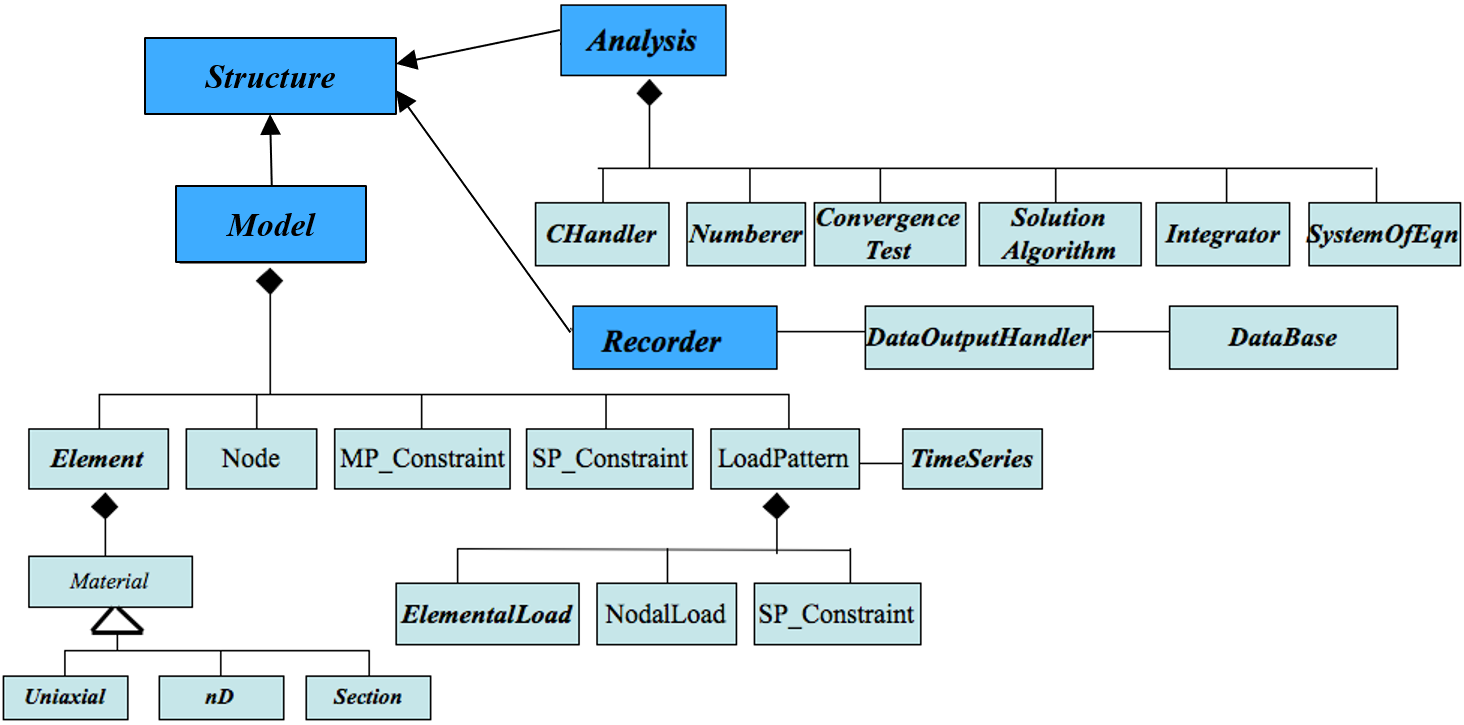
\includegraphics[scale=0.60]{domain.png}
		\centering
		\caption{OpenSees Abstraction}
		\label{fig:abstraction}%
	\end{figure}

	The key domains are formalized by the OpenSees authors as:
	\begin{itemize}
		\item \textit{Model}: This domain contains the information regarding the structure to be modeled, see Fig.~\ref{fig:os_model}. A structure can be idealized as a collection of nodes and elements. The node represents the joints of the structure and the element describes the structural member that connects the nodes. If necessary nodes may have constraints to emulate the boundary conditions. Each element has their own geometirc properties (section dimensions)  and materials (steel, concrete, etc.). Finally, the loading patterns (what is the magnitude and direction of the load and where does it apply) can be defined in this domain. While in meta-modeling the patterns are assumed to be part of modeling domain, it is always associated with analysis to streamline the transformation from model to script.
		\item \textit{Analysis}: The analysis domain contains the parameters related to solver mechanisms, convergence algorithms, etc. User can decide whether to run static or transient analysis.
		\item \textit{Recorder}: This domain handles saving the simulation results to harddrive or to a adatabase. The results can be saved as a xml file or plain text. Node or element responses can be captured using recorders. Plain text does not provide metadata in the header. Therefore, this project relies on xml version.
	\end{itemize}

	There are also utility functions provided by OpenSees to ease the workflow during writing scripts.

	\begin{figure}[htbp]
		% trim={<left> <lower> <right> <upper>}
		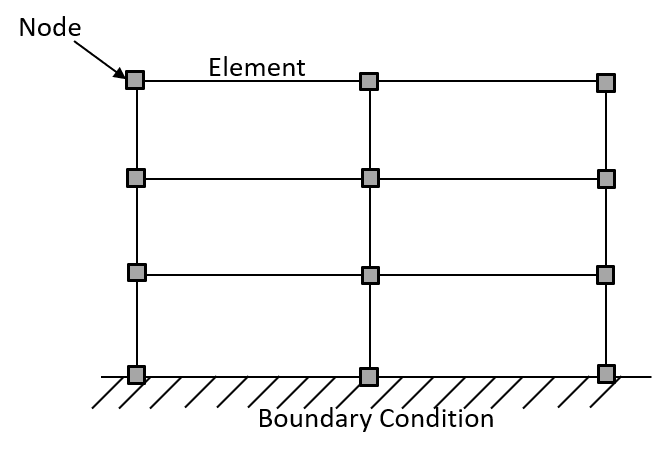
\includegraphics[scale=0.60]{model.png}
		\centering
		\caption{Idealization of the Structure}
		\label{fig:os_model}%
	\end{figure}
	
	\section*{Brief Summary on Implementation}
	One can run a simulation by coding the structure using the three domains explained above. Meta-modeling allows users to describe the structure using building blocks. Each building block in the meta-model is associated with script pieces. For example \textbf{node} block in the meta-model corresponds to \textbf{node} script. This tool encapsulated a major portion of the scripts documented in the OpenSees website.
	
	\subsection*{Meta-Model}
	The meta-model has three domains similar to OpenSees abstraction (\textit{Modeling, Analysis, Recorder}). Additionally, a \textit{Misc.} domain is defined that contains essential OpenSees utility function. Last but not least, the Meta-Model has its own utility domain that contains blocks such as Documentation and MetaData. Additionally, \textit{constants} is defined here which is not part of OpenSees model but part of Tcl scripting scheme, see \url{https://wiki.tcl-lang.org/page/constants}.
	
	\subsection*{Composition}
	There are over 80 components in this meta-model including the abstract nodes.	The compositions are structured in such a way that there each domain has a number of abstract components and the derivatives from those components. For example, \textbf{algorithm} is an abstract component in the domain analysis which is responsible for defining the solution algorithm.  There are five algorithm types user can pick from such as \textbf{algorithm Linear}, \textbf{algorithm Newton} and so on. This pattern is pursued for all the major compositions. However, there are other components which does not need to be identified as abstract.
	
	\subsection*{Transformation}
	Using WebGME, a transformation plugin, \textbf{OpenSeesTransformation} is written. This plugin performs the following operations:
	\begin{itemize}
		\item It transforms the structure (modeled with meta-model blocks) into OpenSees Tcl script input file.
		\item It runs the simulation by executing OpenSees.exe using the generated script file.
		\item The results are written automatically by the OpenSees.exe. This file is used as the base to create json file for the visualizer. Upto this point, Python is used for the transformation.
		\item Using plotly.js the json file is visualized in webGME.
	\end{itemize}
	   
	
	\subsection*{Examples}
	There are two examples are provided within this tool.
	\begin{itemize}
		\item \textit{2D Elastic Structure Static}: This example considers push-over analysis of a three story three bay structure. This model has 16 nodes, and 21 elements. The structure is fixed to the ground. For  horizontal elements (beams), a linear geometric deformation is assumed. As for the vertical elements (columns), P-Delta effect (a common assumption for analysis of structures subjected to lateral loads) is assumed for realistic simulation.
		This structure has two combined and subsequent simulations to emulate a realistic responses. First, a gravity load is applied on the beams to emulate structural weight. The second simulation is a push-over analysis, where a lateral load is applied on the nodes. Both analysis are static, i.e. inertial forces are ignored.
		A recorder is defined to capture the lateral response of the structure to the applied lateral load for the nodes 5-15. Nodes 1 to 4 are fixed hence they don't move and there is no need to record their responses.
		\item \textit{2D Elastic Structure Dynamic}: This example considers transient analysis of the same structure under the influence of ground motion. 
		This example has also two combined and subsequent simulations. First, a gravity load is applied on the beams to emulate structural weight. This simulation is static. The second simulation is a transient analysis, where ground motion recorded by a nearby station during 1995 Kobe earthquake is applied from the ground.
		A recorder is defined to capture the lateral response of the structure during the simulation.
	\end{itemize}
	
	\section*{Using Repo}
	Below, the steps are explained to run open OpenSees Meta-Model tool.
	
	\begin{itemize}
		\item Follow the standard installation and setup of WebGME (as instructed here \url{https://github.com/webgme/webgme}).
		\item The project assumes your mongodb folder is \textbf{webgmeData} under C drive and your application folder is \textbf{mywebgmeapp} under C drive.
		\item There is a plugin called OpenSeesTransformation that converts an OpenSees WebGME model into Tcl script. It is located under \url{src/plugins/OpenSeesTransformation}. Standard entry point for debug is \textbf{run\_debug.py} under the same folder. The transformation code is given in \textbf{init.py} under \url{src/plugins/OpenSeesTransformation/OpenSeesTransformation}
		\item Python 3.6 is used. Packages like webgme\_binding, sys, os, time, csv, subprocess, signal, atexit, ElementTree, StringIO and logging should be already installed since the transformation code.
		\item plotly.js is used for visualization. It is already provided in the repo so no need for new installation.
		\item Dumping the content to a freshly created \textbf{mywebgmeapp} should make the project work.
	\end{itemize}

	\section*{Running Transformation}
	\begin{itemize}
		\item There are two examples. One for 2D (pushover) static and the other one is dynamic (earthquake) simulation.
		\item Click on the example that you want to play with. Select validPlugins as OpenSeesTransformation if not selected.
		\item Open the example double-clicking on it. Do not click on any block and run OpenSees transformation.
		\item Under a minute, the plugin will convert the model into an executable Tcl script, run the simulation, and generate outputs.
		\item After successful run of the plugin, go to \textbf{SimulationResultPlotter} under Visualizer Selector on the left side. This will show simulation results. The visualization may take some a minute due to the amount of data.
	\end{itemize}

\end{document}